\documentclass{ifri}

\setlength{\glsdescwidth}{0.65\textwidth}
% \usepackage{lscape}

\typeMemoire{Diplôme de Licence en Informatique}
\optionFormation{Sécurité Informatique}
\etudiant{Jospy \textbf{GOUDALO}}
\titreDuMemoire{Proposition d'un syst\`eme de paiement \'electronique des factures d'\'electricit\'e de la SBEE.}

\dateSoutenance{-}
%\promo{2\up{ème}}
\anneeScolaire{2017-2018}

%%maitre de mémoire
\encadrants{\textbf{Professeur Eugène C. EZIN}\\Maître de Conférences en Informatique\\Université d'Abomey-Calavi}

\hypersetup{
 pdftitle={Proposition d'un syst\`eme de paiement \'electronique des factures d'\'electricit\'e de la SBEE.},
 pdfauthor={Jospy GOUDALO, jospygoudalo@gmail.com},
 pdfsubject={Proposition d'un syst\`eme de paiement \'electronique des factures d'\'electricit\'e de la SBEE.},
 pdfkeywords={système, paiement, factures, electriques, SBEE} 
 }

\color{bookColor}

%importation du glossaire
\loadglsentries{glossaire/glossaire_reduit}

\begin{document}

\pageDeGarde
%\pageTitre

\pagecolor{white}

%% page vide
%\thispagestyle{empty}\ \clearpage

\selectlanguage{french}

% sommaire
\pagenumbering{roman}

\tableofcontents
\newpage

%liste des figures
\listoffigures 

%liste des tableaux
\listoftables

%liste des algo
\selectlanguage{french}
%\listofalgorithms

% Les sigles et acronymes
\setglossarystyle{super}
\printglossary[title=Sigles et Abréviations, toctitle=Sigles et Abréviations, type=\acronymtype]

% Le glossaire proprement dit
\setglossarystyle{altlist}
\printglossary[type=main]

%% rdedicaces
\dedicace

\paragraph{}
	\begin{center}
		A    
	\end{center}
	\subparagraph*{\\ \\}
	\begin{center}
	 mon Père  \textbf{Noll GOUDALO} 
	\end{center}
	\begin{center}
    ma Mère  \textbf{Nadine SODEDJI}  
	\end{center}
	\begin{center}
      et mon Frère \textbf{Brice GOUDALO}
	\end{center}


 

%% remerciements
\remerciements


\paragraph{}
      Nous exprimons notre vive gratitude aux personnes physiques et institutions qui ont contribué à rendre meilleur notre travail,
   notamment :
  \begin{itemize}
   \item M. Eugène C. EZIN,  notre Maître de mémoire et Directeur de l'Institut de Formation et de Recherche en Informatique (IFRI);
   \item M. Armand ACCROMBESSI, D\'eveloppeur et enseignant à l'IFRI;
   \item Tous les enseignants de l'IFRI pour nous avoir donn\'e les enseignements n\'ecessaires tout au long de notre formation;
   \item M. Camille METINHOUE, Directeur des Syst\`emes d'Information de la SBEE;
   \item M. Idriss SANTANNA et M. Arron ALLADAYE, mes encadreurs  de stage respectivement Chef Service Syst\`eme, S\'ecurit\'e et Maintenance des Infrastructures et Chef Service R\'eseaux T\'el\'ecommunications et TIC \`a la  Direction des Syst\`emes d'Information de la SBEE;
   \item Tout ceux du personnel de la SBEE qui nous ont apport\'es leur soutien tout au long de notre stage;
  \end{itemize}
    Que tous ceux qui nous ont aidé, de près ou de loin, trouvent ici l'expression de nos sentiments les meilleurs.

%\newpage 

% Résume
\resume
\selectlanguage{french}
\begin{abstract}
Resume en francais

\paragraph{}
\textbf{Mots clés}: s\'ecurit\'e ,paiement, factures, sbee, 
\end{abstract}

\newpage
\selectlanguage{english}
\begin{abstract}

Resume en anglais

\paragraph{}
\textbf{Key words}: ....,....,....
\end{abstract}





\pagenumbering{arabic}
\setcounter{page}{1}
%%introduction
\introduction
    \paragraph{}
      \small{
      L'informatique, science du traitement rationnel et automatisé de l'information, est devenue aujourd'hui un outil indispensable pour l'évolution de toute nation, de toute société. Elle est passée d'un statut luxueux à un statut nécessaire. La preuve : toute structure de renom investit un budget non n\'egligeable pour l'informatisation de ses opérations. Cependant, certains sont ne sont toujours pas en phase avec l'\'evolution de la technologie en rapport avec les services qu'ils offrent et la s\'ecurit\'e de ces derni\`eres. Dans le m\^eme temps, des individus profitent de ce ph\'enom\`ene pour pi\'eger les autres ignorant le fonctionnement de l'ordinateur ou non dans le but de voler ou alt\'erer des informations précieuses et confidentielles pour des fins diverses : c'est la cybercriminalité. Vu l'ampleur que prend ces diff\'erents crimes, il devient n\'ecessaire de voir autrement l'importance de la s\'ecurit\'e dans tous les syst\`emes d'informations.
    
    \section{Contexte et justification}
    
	Le Bénin s’inscrit depuis quelques années dans une politique de restructuration du secteur numérique pour y insuffler une nouvelle dynamique. Plusieurs projets et programmes sont donc nés de cette volonté et constituent une feuille de route pour les acteurs au cœur de cette restructuration. 
	\\Dans l'optique de contribuer au d\'eveloppement de ce secteur et surtout de faciliter la vie \`a la population b\'eninoise, nous avons pens\'e \`a mettre en place une plateforme permettant le paiement \`a distance des factures d'\'electricit\'e de la SBEE. Cependant, il s'agit d'un syst\`eme assez critique lorsque nous consid\'erons la quantit\'e et la criticit\'e/le caractère critique  du flux d'informations que nous aurons \`a traiter. La sécurité de l'information revêtant une importance capitale pour la survie d'un peuple, il faudra aussi mettre en oeuvre un système de défense face aux menaces pour réduire l'impact des attaques et essayer, au maximum, d'éliminer les risques. Un aucun aspect ne doit \^etre pris \`a la l\'eg\`ere.
	}
    
    \section{Problématique}
    \small{
	Il n'est plus \`a d\'emontrer que l'\'electricit\'e est \`a la base de tout d\'eveloppement. De la disponibilité de l’énergie dépend la satisfaction de tous les besoins humains fondamentaux : l’eau, l’alimentation, la santé, l’éducation. L'option la plus accessible est de souscrire \`a un abonnement post-pay\'e avec la SBEE.
	N\'eanmoins il n'est pas rare de constater qu'apr\`es de longues heures d'attente au guichet de la SBEE, l'on vous dise: ``D\'esol\'e monsieur nous avons un probl\`eme de connexion. Veuillez repasser demain.''. Il faudra donc repasser plus tard pour solder la facture alors que nous n'avons pas forc\'ement assez de temps pour cela. \\
	Nous sommes aussi parfois confront\'es \`a l'oubli des factures non pay\'ees. Cependant quand vous n'\^etes pas \`a jour apr\`es un d\'elai d'environ un mois, un agent peut passer \`a tout moment couper le courant et vous devez payer des p\'enalit\'es. Notre travail consistera donc \`a mettre en place une application web permettant le paiement des factures depuis un t\'el\'ephone portable ou un ordinateur connect\'e \`a Internet. Cependant les donn\'ees g\'erees par cette application sont sensibles et critiques. A titre d'exemple les informations de votre carte VISA\footnote{Carte de paiement émise par l'établissement bancaire de son titulaire} pourraient \^etre vol\'ees. La carte sera donc utilis\'ee \`a votre insu et votre argent ne vous appartiendra plus. Il sera donc nécessaire de prendre en compte toutes les menaces possibles et d'y apporter des solutions efficientes. Ainsi nous pourrions avoir une application s\'ecuris\'ee permettant le paiement des factures \'electriques depuis un appareil connect\'e \`a Internet.
	}

    \section{Objectifs}
    \small{ 
	  Notre projet a pour objectif principal de faciliter le paiement des factures \'electriques de la SBEE et de mettre en place les garde four nécessaire pour réduire les attaques informatiques.
	        
	  Plus précisément, il s'agira de :
	
    \begin{itemize}
	\item Rappeler aux personnes utilisant la plateforme qu'ils ont des impay\'es (via des SMS et/ou des emails)
        \item Assurer la disponibilit\'e compl\`ete de la plateforme afin que les consultations et paiements puissent se faire \`a n'importe quel moment.
	\item Garantir la s\'ecurit\'e de toutes les transactions financi\`eres effectu\'ees via la plateforme
	\item Construire un historique afin d'avoir une trace des factures pay\'ees et impay\'ees ainsi que des d\'epenses.
    \end{itemize}
    }

    \section{Environnement de stage}
      \small{
	Ce travail \`a \'et\'e r\'ealis\'e dans les locaux de la Direction des Syst\`emes Informatiques (DSI) de la Soci\'et\'e B\'eninoise d'Energie Electrique (SBEE) - Direction G\'en\'erale. La SBEE a pour mission de produire, de transporter et de distribuer l’énergie électrique sur l’ensemble du territoire national. Elle a son siège social à Cotonou - Ganhi et couvre le territoire national à travers  huit (8) Directions Régionales et trente-neuf (39) agences géographiquement réparties dans tous les départements du pays.
      }
      
    \section{Organisation du mémoire}
	\small{
	  Le présent travail se présente en trois (03) chapitres. Le premier concerne la revue de littérature sur le syst\`eme existant (actuel) permettant le paiement des factures et quelques notions par rapport \`a la s\'ecurit\'e des applications Web. Le deuxième chapitre aborde les choix organisationnels (proc\'edures) et techniques opérés en vue de la conception et de la réalisation des solutions proposées. Le troisième chapitre, quant à lui, fait une analyse critique des résultats issus de nos tests après les avoir exposés.
	}



%\lhead[]{} \rhead[]{} \chead[]{}
\selectlanguage{french}
\fancyhead[L]{\tiny \leftmark}
\fancyhead[R]{\scriptsize \rightmark}
\fancyfoot[C]{\thepage}

\chapter{Revue de littérature}\label{chap:1}
  \section*{Introduction}
	\paragraph{}
      Pour bien réaliser un projet, un état des lieux permettant de faire un point sur le sujet du projet est requis. Ainsi, ce chapitre présente un état des lieux concernant les intrusions informatiques. Dans un premier temps, nous aborderons les généralités sur les intrusions informatiques, puis nous présenterons quelques solutions existantes.
  \section{Généralités sur les intrusions informatiques}
  \paragraph{}
  D’après LE PETIT LAROUSSE ILLUSTRE 2010, l’intrusion est définie comme <<l’action de s’introduire sans y être invité dans un lieu, une société, un groupe, un système informatique. C’est aussi l’action d’intervenir dans un domaine où l’on n'a aucun titre à le faire>>. Cette définition de l’intrusion s’applique aussi en informatique \footnote{ Le petit Larousse Illustré 2010.} \cite{b}. En effet, l’intrusion en informatique est définie comme étant toute utilisation d’un système informatique à des fins autres que celles prévues, généralement après acquisition de privilèges de façon illégitime.
\paragraph{}
  L'arrivée d'Internet a apporté une grande révolution dans le monde mais aussi a entraîné une kyrielle de problèmes dans le domaine de la protection de la vie privée.  Ainsi des personnes appelées hackers arrivent à prendre possesion de tout un système d'information et à le paralyser.

  
\subsection{Notion de hacker et de cracker}
  \paragraph{}
    Un hacker est une personne qui, par jeu, goût du défi ou souci de notoriété, cherche à contourner les protections d'un logiciel, à s'introduire frauduleusement dans un système ou un réseau informatique. \cite{A} \footnote{Recommandation officielle : fouineur.}.\\Un cracker, quant à lui, s’introduit tout aussi frauduleusement dans un système informatique pour en entraver ou en fausser le fonctionnement. Son action est souvent plus dévastatrice.
	

\subsection{Mode opératoire d'une intrusion informatique}
  \paragraph{}
    Un test d’intrusion peut être décomposé en une suite d’étapes ou phases. Lorsqu’elles sont réunies, ces étapes forment une méthodologie complète pour mener à bien un test d’intrusion. L’établissement d’une méthodologie permet de décomposer une procédure complexe en une suite de tâches gérables de taille plus réduite. Ainsi nous regroupons cette méthodologie en quatre étapes qui sont \textbf{la reconnaissance}, \textbf{les scans}, \textbf{l'exploitation}, \textbf{la postexploitation et le maintien d'accès} \footnote{La post exploitation et le maintien d'accès forment une étape.}\cite{c}.
      
  \subsubsection{La reconnaissance}
    \paragraph{}
      La reconnaissance, ou recueil d’informations, est probablement la plus importante des quatre phases. Plus le hacker passe du temps à collecter des informations sur sa cible, plus les phases suivantes auront une chance de réussir\cite{c}. En effet la reconnaissance permet de connaitre la cible dans les détails, de connaître les points forts et surtout les points faibles afin de notifier les prochaines possibilités d'attaque.

  \subsubsection{Les scans}
    \paragraph{}
      Les scans sont des procédés ayant pour objectif d’identifier les systèmes actifs et les services qui existent sur les systèmes scannés. Dans ce cadre, le hacker prend le soin de vérifier l'activité d'un système, de trouver les portes ouvertes (les ports), de vérifier les processus tournant sur le système et d'aller à la recherche des vulnérabilités. Ce stade requiert une compréhension plus avancée des systèmes informatiques pour mieux comprendre les résultats recueillis \footnote{Informations recueillis au cours du scan}\cite{c}.
      
  \subsubsection{L'exploitation}
    \paragraph{}
      En termes simples, l’exploitation consiste à obtenir un contrôle sur un système. Toutefois, il est à notifier que tout exploit ne conduit pas à la compromission intégrale d’un système. Un hacker peut se servir donc d'un exploit pour télécharger des contenus dont il ne détient pas la propriété pendant qu'un autre utilise un exploit pour crypter les fichiers du système. L'utilisation de l'un des exploits \footnote{Un exploit est le moyen par lequel un attaquant, ou un pentester en l’occurrence, profite d’un défaut dans un système, une application ou un service.} dépend donc de l'objectif visé par le hacker \cite{E}.

  \subsubsection{Post exploitation et maintien d’accès}
    \paragraph{}
      Cette étape consiste à couvrir les traces de l'intrus agissant afin de ne pas se faire repérer \cite{E}. Il permet aussi à ce dernier de facilliter ses prochains accès à la machine victime de ses attaques par l'installation de portes dérobées communément appelées "Backdoor". Ainsi, il n'aura plus besoin de reprendre toutes les étapes de son processus pour accéder à la machine dont il prend le contrôle.\\ \\
      

\begin{figure}[H]
  \begin{center}
    %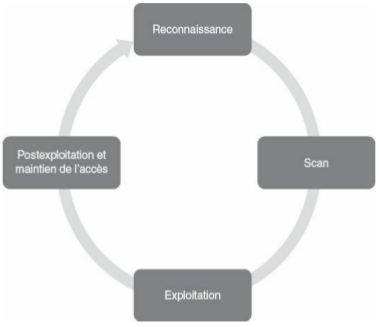
\includegraphics[scale=0.5]{images/zeh_cycle.png}
  \end{center}
  \caption[Représentation cyclique de la méthodologie ZEH.]
    {Méthodlogie ZEH, Patrcick Engebretson, "Les bases du hacking", PEARSON 2013}
    \label{Methodologie d'intrusion}
\end{figure}

\paragraph{}
  La méthodologie d'attaque étant cernée, nous allons maintenant présenter les différentes sortes d'attaque auxquelles sont confontrés les systèmes informatiques.	    
		    
\subsection{Quelques exemples d'attaques informatiques}
  \paragraph{}
    Parmi les attaques les plus connues, on peut citer les techniques de déni de service (DoS), l'usurpation d'adresse IP, l'usurpation du DNS \textit{Domain Name Server}, l'ingénierie sociale.		    
	
  \subsubsection{Le deni de service}
    \paragraph{}
      D'une manière générale, on parle de déni de service quand une personne ou une organisation est privée d'un service utilisant des ressources qu'elle est en droit d'avoir en temps normal \cite{B}. On trouvera par exemple des dénis de service touchant le service de courrier électronique, d'accès à Internet, de ressources partagées (pages Web), ou tout autre service à caractère commercial comme Yahoo ou EBay.\\ \\
      Quoiqu'il en soit, le déni de service est un type d'attaque qui coûte généralement très cher puisqu'il interrompt le cours normal des transactions pour une entreprise; les sommes et les enjeux sont énormes et cela ne peut aller qu'en s'aggravant tant que des parades réellement efficaces n'auront pas été trouvées.\\ \\
      Il existe plusieurs moyens pour parvenir à un déni de service. Nous ne parlerons que de trois types dont l'attaque avec les paquets \textbf{XMAS}, l'attaque \textbf{Smurf}, et l'attaque par \textbf{Syn flooding}.

      \subparagraph*{L'attaque avec paquets XMAS.}
	Un paquet XMAS ou Christmas Tree est un paquet dans lequel les drapeaux \textit{(flag)} de tout protocole sont définis. Les bits FIN, URG et PSH dans l'en-tête TCP de ce type de paquet sont définis. Ce paquet s'appelle paquet Christmas Tree, car tous les champs d'en-tête sont éclairés c'est à dire activés comme un arbre de noël. Ce type de paquet nécessite beaucoup plus de traitements que les paquets habituels, de sorte que le serveur alloue un grand nombre de ressources pour ce paquet. Par conséquent, cela peut être utilisé pour effectuer une attaque DoS sur le serveur.

      \subparagraph{L'attaque Smurf.}
	L'attaquant ici envoie un grand nombre de paquets de diffusion d'écho ICMP, avec des adresses IP source falsifiées par rapport à l'adresse IP de la cible. Toutes les machines du réseau reçoivent ce message de diffusion et répondent à la cible avec un paquet de réponse d'écho.

      \subparagraph{Le syn flooding.}
	Lors de l'initialisation d'une connexion TCP entre un client et un serveur, un échange de messages a lieu. Le principe est celui du three-way handshake, qui dans le cas d'une connexion normale sans volonté de nuire, se déroule en trois étapes :
	\begin{enumerate}
	  \item le client demande une connexion en envoyant un message SYN (pour synchronize) au serveur;
	  \item le serveur accepte en envoyant un message SYN-ACK (synchronize-acknowledgment) vers le client;
	  \item le client répond à son tour avec un message ACK (acknowledgment) ; la connexion est alors établie.
	\end{enumerate}
	
	\begin{figure}[H]
	  \begin{center}
	    %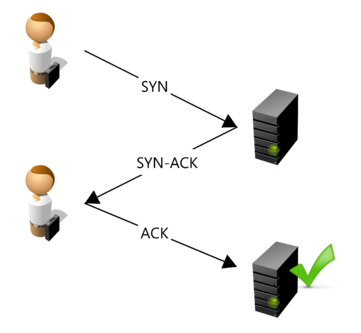
\includegraphics[scale=0.5]{images/handshake.png}
	  \end{center}
	  \caption[TCP handshake]{3 ways Handshake}
	  \label{Mécanisme d'établissement de connexion TCP}
	\end{figure}
	
	L'attaquant peut créer un grand nombre de requêtes SYN forgées qui ont leurs adresses IP source falsifiées et l'envoyer à la cible. La cible répond avec SYN-ACK et alloue ses ressources pour la connexion, mais ne reçoit jamais la réponse ACK. Les ressources de la machine cible sont épuisées et elles ne permettent pas de répondre à d'autres demandes de  machines légitimes.

	\subsubsection{L'usurpation d'adresse IP}
	  \paragraph{}
	    L'« usurpation d'adresse IP » (également appelée mystification ou en anglais \textit{IP Spoofing}) est une technique consistant à remplacer l'adresse IP de l'expéditeur d'un paquet IP par l'adresse IP d'une autre machine.
	    Cette technique permet ainsi à un pirate d'envoyer des paquets de façon anonyme. Il ne s'agit pas pour autant d'un changement d'adresse IP, mais d'une mascarade de l'adresse IP au niveau des paquets émis \cite{F}.

	\subsubsection{L'usurpation DNS}
	  \paragraph{}
	    Il s'agit de corrompre le cache du serveur DNS \textit{ Domain Name Server} afin de faire croire à une machine qu'un nom de machine est relatif à une fausse adresse donnée. Ainsi donc les communications vers la machine ciblée sont redirigées vers celle dont l'adresse est portée en avant.

	\subsubsection{Ingénierie sociale}
	  \paragraph{}
	  L'ingénierie sociale est une attaque qui s'appuie essentiellement sur les relations humaines pour inciter de façon détournée à enfreindre les procédures de sécurité \cite{social}. L’ingénierie sociale fait partie des techniques les plus simples, mais aussi les plus efficaces pour entrer dans un système sécurisé à grande échelle. En effet le système aura beau être sécurisé avec les moyens les plus sophistiqués, une seule information divulguée d'un utilisateur aura suffi pour mettre le système à terre. Il s'agit d'une arme très forte résultant de l'étude de l'être humain, de ses passions, de ses désirs. Cette forme d'attaque est très dévastatrice en fonction de l'importance des informations tirées.\\
	  Face à ces différentes menaces, différentes solutions sont nées. Nous allons en présenter quelques-unes.
		        	    
    \subsection{Les applications basées sur la détection et la prévention d'intrusion}
      \paragraph{}
	Plusieurs systèmes ont vu le jour en raison des attaques qui sévissent de jour en jour. Il s'agit des IDS (\textit{Intrusion Detection System}), des IPS (\textit{Intrusion Prevention System}), des firewall (Pare-feu), des antivirus pour ne citer que ceux là.
	
      \subsubsection{Les systèmes de détection d'intrusion}
	\paragraph{}
	  Un système de détection d’intrusion \textit{Intrusion Detection System (IDS) en anglais} est comparable à une alarme domestique contre les voleurs. Si une tentative de pénétration non avenue est découverte, une alerte sera déclenchée.
	  La fiabilité d'un tel système dépend de la puissance des capteurs à détécter les événements pour lequels ils ont été mis en place avec une marge d'erreur minimisée. 
	  Certains termes sont souvent employés quand on parle d’IDS et il sied de les  comprendre. Il s'agit notamment du faux positif et du faux négatif.\\
	  Un faux positif est une alerte provenant d’un IDS mais qui ne correspond pas à une attaque réelle, tandis qu'un faux négatif est une intrusion réelle qui n’a pas été détectée par l’IDS.

    Un systéme de détection d'intrusion se base sur trois éléments particuliers:
    \begin{itemize}
      \item la sonde qui collecte les informations sur le système;
      \item l'analyseur qui traite ces informations afin de détecter les possibilités d'attaque;
      \item la réponse qui est la solution apportée à la menace détectée.
    \end{itemize}    

    \textbf{Quelques exemples d'IDS}
    
  \begin{itemize}
    \item \textbf{Snort}\\
      Pour effectuer ces analyses, Snort se fonde sur des règles \cite{d}. Snort est fourni avec certaines règles de base mais cependant, comme tout logiciel, Snort n'est pas infaillible et demande donc une mise à jour régulière. Snort peut également être utilisé avec d'autres projets open sources tels que SnortSnarf, ACID, sguil et BASE (qui utilise ACID) afin de fournir une représentation visuelle des données concernant les éventuelles intrusions.

    \item \textbf{Bro}\\
      Bro s'appuie sur les mêmes bases théoriques que Snort (filtrage par motif, formatage aux normes RFC, etc), mais il intègre un atout majeur : l'analyse de flux réseau. Cette analyse permet de concevoir une cartographie du réseau et d'en générer un modèle. Ce modèle est comparé en temps réel au flux de données et toute déviance lève une alerte \cite{h}.

    \item \textbf{Fail2ban}\\
      Fail2ban bloque les adresses IP appartenant à des hôtes qui tentent de casser la sécurité du système. Il lit les logs de divers services (SSH, Apache, FTP…) à la recherche d'erreurs d'authentification répétées et ajoute une règle iptables pour bannir l'adresse IP de la source \cite{i}.
  \end{itemize}

      \subsubsection{Les systèmes de prévention d'intrusion}
	\paragraph{} 
	  Le besoin de ne pas attendre les attaques avant de réagir s'est ressenti, compte tenu des inconvénients générés par ces attaques. C'est ainsi que sont nés les IPS \textit{Intrusion Prevention System}. Ces derniers utilisent des techniques qui permettent de surveiller les processus d’un système et de tuer ceux dont le comportement paraît douteux tel que les processus qui tentent d’exécuter un dépassement de tampon. Cependant, quelques risques sont liés à leur utilisation. Il s'agit en particulier de l'arrêt des processus mis en activité par l'utilisateur, ce qui devient une restriction anormale.
		
    \textbf{Quelques exemples d'IPS \cite{e}}
    \begin{itemize}
      \item \textbf{Suricata}\\
	Suricata est un logiciel open source de prévention d'intrusion et de supervision de sécurité réseau. Il est développé par la fondation OISF \textit{Open Information Security Foundation} \cite{G}.

      \item \textbf{Snort Inline}\\
	L'IPS Snort Inline est une version modifiée de l'IDS Snort pour en faire un IPS, une solution capable de bloquer les intrusions ou attaques réseau. Il reçoit les paquets envoyés par le firewall Netfilter avec l'aide de la librairie libipq, les compare avec des règles de signature Snort et les marque en drop s'ils correspondent à une règle, puis finalement les renvoie vers Netfilter où les paquets Snort Inline marqués sont rejetés \cite{d}.

      \item \textbf{HLBR}\\
	HLBR est un système de prévention des intrusions. Sa principale caractéristique est qu'il peut s'exécuter directement sur la couche du modèle OSI, ce qui signifie qu'il n'a même pas besoin d'une pile TCP/IP fonctionnant comme un pont \cite{H}.
    \end{itemize}
    
    \subsubsection{Classification des IDS selon leur emplacement}
      \paragraph{}
	On distingue deux types d'IDS: les HIDS \textit{Host Intrusion Detection System} et les NIDS \textit{Node Intrusion Detection System}.
	Les premiers sont remarquables par leur emplacement sur les machines qu'elle protège. Les seconds se ramarquent par leur position en des points stratégiques du réseau permettant ainsi de surveiller les activités du réseau et d'apporter une protection à l'ensemble du réseau. 	  
			  
    \subsubsection{Les pare-feux}	   
      \paragraph{}
	Les pare-feux sont des systèmes dont le but principal est de limiter le trafic sur un réseau informatique. Ainsi donc, l'administrateur définit les types de trafic voulus et ceux indésirés. A la rencontre d'un trafic non désiré, les paquets relatifs sont rejetés.
	    
    \subsubsection{Les antivirus}
      \paragraph{}
	Les antivirus sont des programmes dont le rôle est de vérifier que  l’identité des arrivants ou des programmes s’exécutant n’existent pas dans une liste noire prédéfinie dans une base de données. On parle de signature. Ainsi donc, la puissance d'un antivirus est basée sur la pertinence des informations contenues dans la base de données qu'il faut mettre à jour régulièrement. 
		 
		  
\section*{Conclusion}
  Les attaques informatiques sont nombreuses et de différentes formes. Dans ce chapitre, nous avons présenté le fonctionnement de quelques unes d'entre elles et exposer certaines solutions existantes. Dans le chapitre suivant, nous aborderons notre solution à travers sa conception et les outils utilisés pour sa réalisation.
 
\chapter{Conception et Matériels}\label{chap:2}
    \section*{Introduction}
  \paragraph{}
	La programmation d'une application requiert d'abord l'organisation et la documentation de ses idées. La définition des modules induit les différentes étapes de sa réalisation. C'est cette démarche antérieure à l'écriture que l'on appelle modélisation. Ainsi, notre modélisation est axée autour de deux diagrammes: le diagramme des cas d’utilisation recense les différentes fonctionnalités de notre système; le diagramme de séquence illustre le fonctionnement interne du système dans le temps.
    
  \section{Conception}
    \subsection{Méthode de modélisation}
      \paragraph{}
      Afin de modéliser les fonctionnalités de notre solution, nous avons choisi le langage UML \textit{Unified Modeling Language} \cite{I}. Issu d’un large consensus, le langage UML garantit la stabilité et la performance d’un projet grâce à son caractère formel et industrialisé. Aussi facilite-t-il la compréhension du système par l’usage de représentations graphiques appelées diagrammes. Ces diagrammes nous ont permis de modéliser notre solution en utilisant les diagrammes de cas d’utilisation et de séquence.\\ \\
\subsection{Diagramme de cas d'utilisation}
    \paragraph{}
	  Le diagramme de cas d'utilisation représente la structure des grandes fonctionnalités nécessaires aux utilisateurs du système. C'est le premier diagramme du modèle UML, celui où s'assure la relation entre l'utilisateur et les objets que le système met en œuvre. 

	  \begin{figure}[H]
		     \begin{center}
			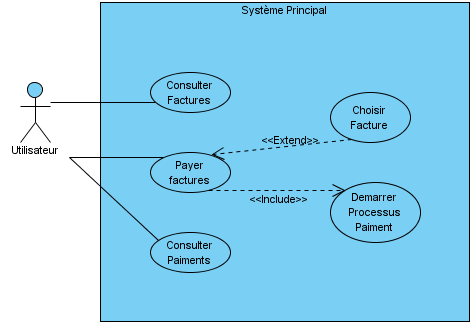
\includegraphics[scale=0.5]{images/uc.png}
		     \end{center}
		     \caption{Diagramme de cas d'utilisation}
		     \label{Diagramme de cas d'utilisation}
	  \end{figure}
	  
	  Pour une premi\`ere utilisation, il est n\'ecessaire de cr\'eer un compte. Les informations \`a fournir sont: un nom, un email, un num\'ero de t\'el\'ephone, la r\'ef\'erence abonn\'ee\footnote{trouver le sens exact} et le mot de passe pour la protection du compte. Ces informations \'etant obligatoires. Un mail d'activation est envoy\'e et l'utilisateur apr\`es activation de son compte peut se connecter \`a l'application. Une authentification est nécessaire afin d'avoir acc\`es aux cas d'utilisations de notre diagramme (ou aux fonctionnalités de l'application).
	  
\subsection{Diagramme de séquence}
 \paragraph{}
	  Le diagramme de séquence représente la succession chronologique des opérations réalisées par un acteur. Ce mode de représentation effectue la description du fonctionnement dynamique du système. En d'autres termes, il indique les objets que l'acteur va manipuler et les opérations qui font passer d'un objet à l'autre.
	  \begin{figure}[H]
		     \begin{center}
			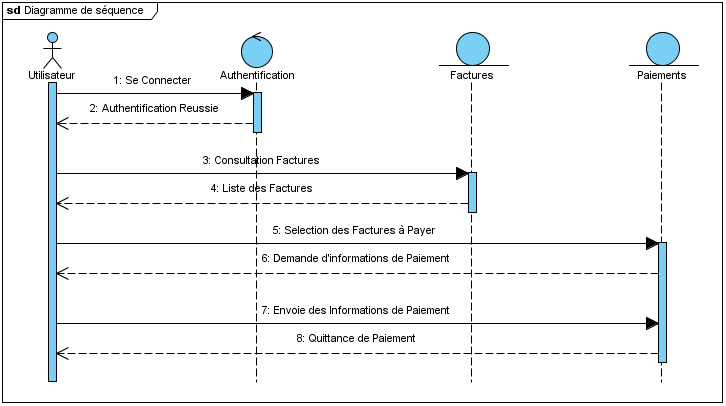
\includegraphics[scale=0.6]{images/sd.png}
		     \end{center}
		     \caption{Diagramme de séquence}
		     \label{Diagramme de cas d'utilisation}
	  \end{figure}
	  Après que l'utilisateur ait entré ses informations, identifiants pour se connecter, il a acc\`es aux factures. L\`a il peut ajouter les factures impay\'ees \`a la liste des factures \`a payer (m\^eme concept que le panier d'un site d'e-commerce). Il pourra donc proc\'eder au paiement de ses factures via le mode de paiement qui lui convient. Une quittance lui est g\'en\'er\'ee et est ajout\'ee \`a son historique de paiements.
  \section{Matériels}
      \subsection{Principe de fonctionnement de notre solution}
      \paragraph{}
	  Nos objectifs pour ce travail sont, dans un premier temps, d'arriver à détecter l'espionnage par webcam et dans un second temps de proposer des options à activer pour protéger l'ordinateur hôte de quelques intrusions qui pourraient survenir. La présentation des principes de fonctionnement se fera en deux étapes: le principe de détection d'attaques par webcam et le principe de protection contre les intrusions.
	  
	  \subsubsection{La webcam}
	  \paragraph{}
	  	Pour détecter l'utlisation illicite d'une ressource, il revient de monitorer en temps réel les flux provenant de cette ressource et générés par des processus. Ainsi, notre solution permet de surveiller les flux de la webcam à intervalles de temps réguliers de trois secondes pour ne pas utiliser, de façon incontrolée, les ressources de l'ordinateur. \\ 
	  	A la découverte d'un processus utilisant la webcam, une alerte est envoyée à l'utilisateur qui choisit si oui ou non il est à la base de l'activité d'un tel processus. Si sa réponse est négative, alors il est victime d'un espionnage et, à ce moment un filtre est fait pour connaitre l'identifiant du processus qui est immédiatement tué. En cas de réponse positive de l'utilisateur (oui c'est bien moi), alors le processus en cours est laissé et la detection de processus utilisant la webcam est désactivée pendant cinq minutes. L'algorithme 1 présente le processus de détection d'espionnage par webcam.
					
%\newpage		
						\begin{algorithm}[H]
						\caption{Algorithme de détection d'espionnage par webcam}
\DontPrintSemicolon % Some LaTeX compilers require you to use \dontprintsemicolon instead

\For{\textit{chaqueTroisSecondes}} {
$etatWebcam \gets enUtilisation()$\;
  \If{$etatWebcam = ouvert$ } {
    $action \gets etesVousAuteur()$\;
     \eIf{$action = non$ } {
    	\textit{chercherIdProcessus()}\;
    	\textit{arreterProcessus()}\;
  }{
	\textit{cinqMinutesDePause()}\;  
  }
  }
}
\Return{$action$}\;
\label{algo:webcam}
\end{algorithm}  		
	  	 
	  	 \subsubsection{Les intrusions }
      \paragraph{}
	   Quand un pirate arrive à prendre possession d'une machine dans un réseau, c'est qu'il est arrivé à établir une connexion entre sa machine et la victime. Ainsi, dans la liste des connexions établies (ESTABLISHED), on peut donc lister la connexion permettant au pirate d'interagir avec sa victime à son insu. Notre solution pour ces attaques est de proposer une option à activer et dont le but est d'alerter l'utilisateur dès qu'une connexion est établie. A cet effet, une vérification des connexions ouvertes se fait toutes les trois secondes. Si l'utilisateur ne reconnait pas cette connexion comme étant légale, alors il le signale par un bouton qu'il appuie et à ce moment, l'adresse source ainsi que le port source de connexion sont mis dans une liste noire. L'algorithme 2 présente les étapes de détection d'intrusions.
	   
	   
						\begin{algorithm}[H]
\DontPrintSemicolon % Some LaTeX compilers require you to use \dontprintsemicolon instead

\For{\textit{chaqueTroisSecondes}} {
$list \gets listeConnexionsEtablies()$\;
	\For{\textit{$connexion$ as $list$}} {
	\textit{alerterConnexionEtablie()}\;
	$action \gets autoriser()$\; 
  \If{$action = non$ } {
   \textit{blacklistAdresseEtPort()}\;
  }
}
}
\Return{$action$}\;
\caption{Algorithme de détection d'intrusions}
\label{algo:intrusion}
\end{algorithm}

Lorsque l'attaque est faite au cours des trois secondes, l'application ne le détecte pas. C'est une de ses faiblesses. 	   
	   \subsubsection{Les whitelist }
      \paragraph{}
	   Il y a des connexions importantes que la machine établit en local avec des adresses locales telle que le 127.0.0.1 qui n'est pas une attaque. Cependant, à l'activation de la détection d'intrusion, notre logiciel alerte l'utilisateur d'une connexion établie en local, ce qui pourrait être considéré comme non importante. C'est ainsi que nous avons proposé une whitelist d'adresses IP où l'utilisateur pourra ajouter ou supprimer les adresses dont il ne s'inquiète pas des connexions établies. Il en est de même pour les ports de connexion tels que le 443 et le 80 qui sont des ports de navigation web. L'utilisateur a donc la possiblité d'ajouter ou de supprimer des ports dans la whitelist, ce qui ne déclenchera plus d'alerte à la découverte d'une connexion avec les paramètres entrés en whitelist. Après avoir modifié la base de données de la whitelist, il faut rafraîchir afin de faire considérer à l'application la nouvelle liste à prendre en compte.
	 	
 		\subsubsection{Les dénis de service}
      \paragraph{}
		Comme nous l'avons présenté au chapitre précédent, un déni de service peut s'effectuer de plusieurs façons. Notre solution, pour cela, propose une option où lorsqu'elle est activée rejette tous les paquets au statut invalide et les paquets avec tous les flags activés (XMAS). Aussi limite-elle le nombre de paquets ICMP à deux (02) par seconde pour eviter les attaques de type Smurf.   
     
	\subsubsection{Limiter le nombre de connexion par adresse}
      \paragraph{}
     Toujours dans l'optique d'arriver à une fin de déni de service, l'attaquant peut falsifier les adresses IP et envoyer des demandes de connexion, la cible peut se retrouver avec une immensité de connexions ouvertes pour une seule adresse. Pour eviter cela, nous proposons à l'utilisateur d'entrer le nombre de connexions maximales qu'il admet pour une adresse IP vers sa machine en dépendance des services qu'il fournit au réseau auquel il appartient. Une fois cette valeur entrée et validée, une règle est créée pour rejeter toute demande de connexion d'une quelconque adresse après avoir atteint la limite entrée par l'utilisateur. Ce dernier a la possibilité de modifier cette valeur à tout moment.    
  \subsection{Langage de développement et outils}
  
      \paragraph{}
	  Notre solution fonctionne sous les systèmes Linux. Cette plate-forme a été choisie en raison de son ouverture, de l'accessibilité au code source et de sa flexibilité. Pour atteindre nos objectifs, nous avons utilisé les langages java, awk et bash; les deux derniers étant des langages de script de Linux. Il est à noter que les versions Debian sont les plus concernées par notre travail. Le tableau suivant fait la synthèse des outils utilisés.
	  
	\begin{table}[H]
	   \begin{center}
	      \caption{Synthèse des outils utilisés}
	      \label{Synthèse des outils utilisés}
		\begin{tabular}{|>{\centering\arraybackslash} p{5cm} |>{\centering\arraybackslash} p{5cm}|>{\centering\arraybackslash} p{5cm}|}
		 \hline
		\begin{bf}Langages\end{bf} & \begin{bf} Systèmes d'exploitation\end{bf} & \begin{bf}Autres Outils \end{bf}\\
		\hline
		\multicolumn{1}{|l|}{Java } & \multicolumn{1}{|l|} {Ubuntu 16.04 LTS}& \multicolumn{1}{|l|}{Iptables }\\
		\hline
		\multicolumn{1}{|l|}{Bash } & \multicolumn{1}{|l|} {Kali Linux 2.0 Rolling}& \multicolumn{1}{|l|}{ }\\
		\hline
		\multicolumn{1}{|l|}{Awk} & \multicolumn{1}{|l|}{} & \multicolumn{1}{|l|}{ }\\
		\hline
		
		\end{tabular}
	   \end{center}
	  \end{table}
	  
	 Les langages et outils présentés dans le tableau sont ceux utilisés pour le développement de notre application pendant que les systèmes d'exploitations présentés sont ceux utilisés pour le cas pratique.

      \subsection{A propos de Debian}
	\paragraph{}
	  Debian est un système d'exploitation libre. Il est simple et est constitué de plus de 4000 paquets. Les paquets sont des composants logiciels précompilés conçus pour s'installer facilement sur la machine hôte. L'ouverture de Debian permet à plusieurs programmeurs de pouvoir identifier les failles de sécurité ou de créer plusieurs modules pour faire des tâches qui s'avèrent indispensables. C'est ainsi que la communauté de Debian devient de plus en plus robuste et flexible. Plusieurs systèmes d'exploitation sont dérivés de Debian dont Kali Linux spécialisé dans les tests d'intrusion. 
  
\section*{Conclusion}
		\paragraph{}
	  Dans ce chapitre, nous avons présenté les choix techniques opérés
	  ainsi que notre solution à travers sa modélisation, son principe de fonctionnement et les outils utilisés. 
	  Le chapitre suivant exposera les différents résultats et quelques critiques.
 
\chapter{Résultats et Discussion}\label{chap:3}
  \section*{Introduction}
    \paragraph{}
    Dans ce chapitre, nous présentons les résultats des simulations faites pour tester le fonctionnement de notre solution. Dans un premier temps,
    nous allons présenter l’application, une attaque pour tester la s\'ecurit\'e de notre r\'eseau et nous aborderons ensuite une discussion.


    \section{Présentation des résultats des tests}
      \paragraph{}
	  \begin{figure}[H]
	      \begin{center}
		  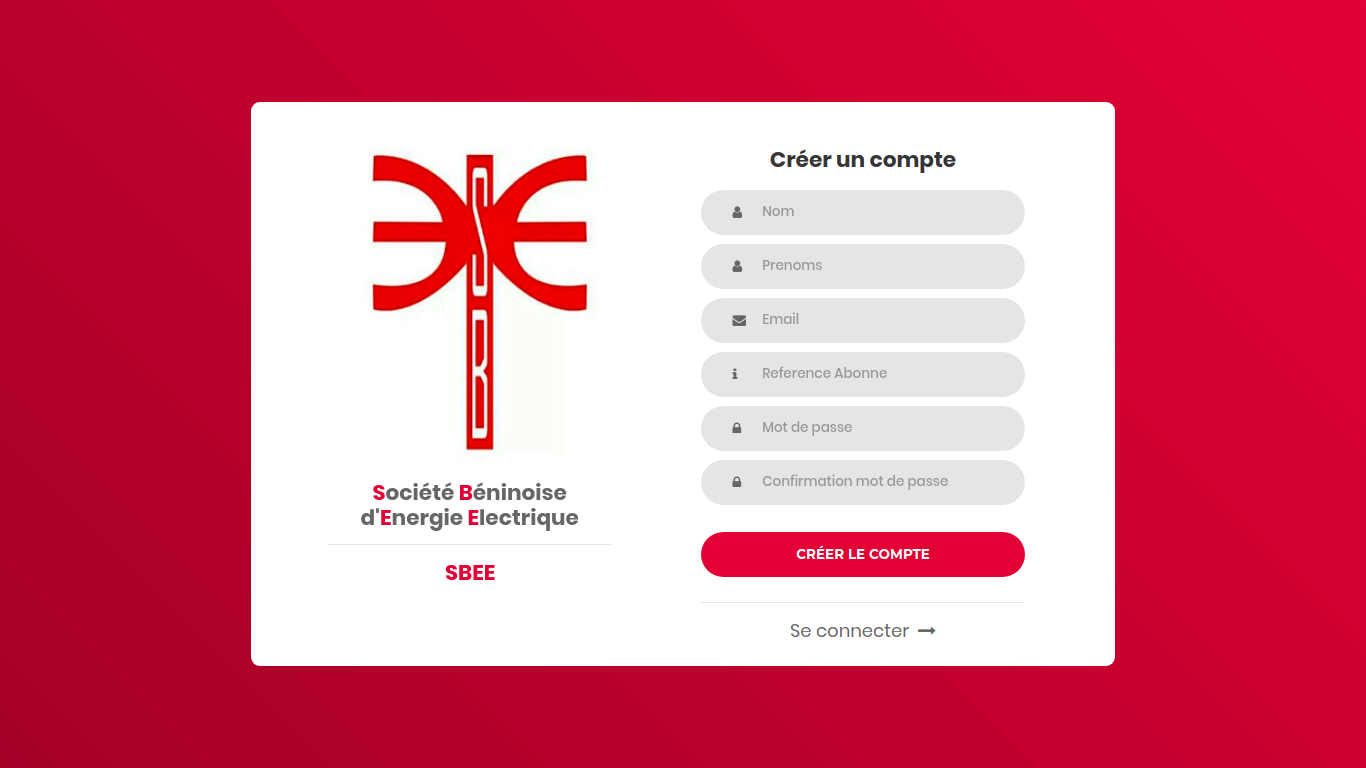
\includegraphics[scale=0.35]{images/register.png}
	      \end{center}
	      \caption{Page d'inscription de l'application}
	      \label{Accueil}
	  \end{figure}
	  La figure 3.1 présente la page d'ouverture de compte de notre application. L'utilisateur entre son nom, pr\'enom(s), adresse email, la r\'ef\'erence abonn\'ee et le mot de passe. Un mail d'activation lui est envoy\'e et il est redirig\'e vers la page de connexion.
	      
	  \begin{figure}[H]
	      \begin{center}
		  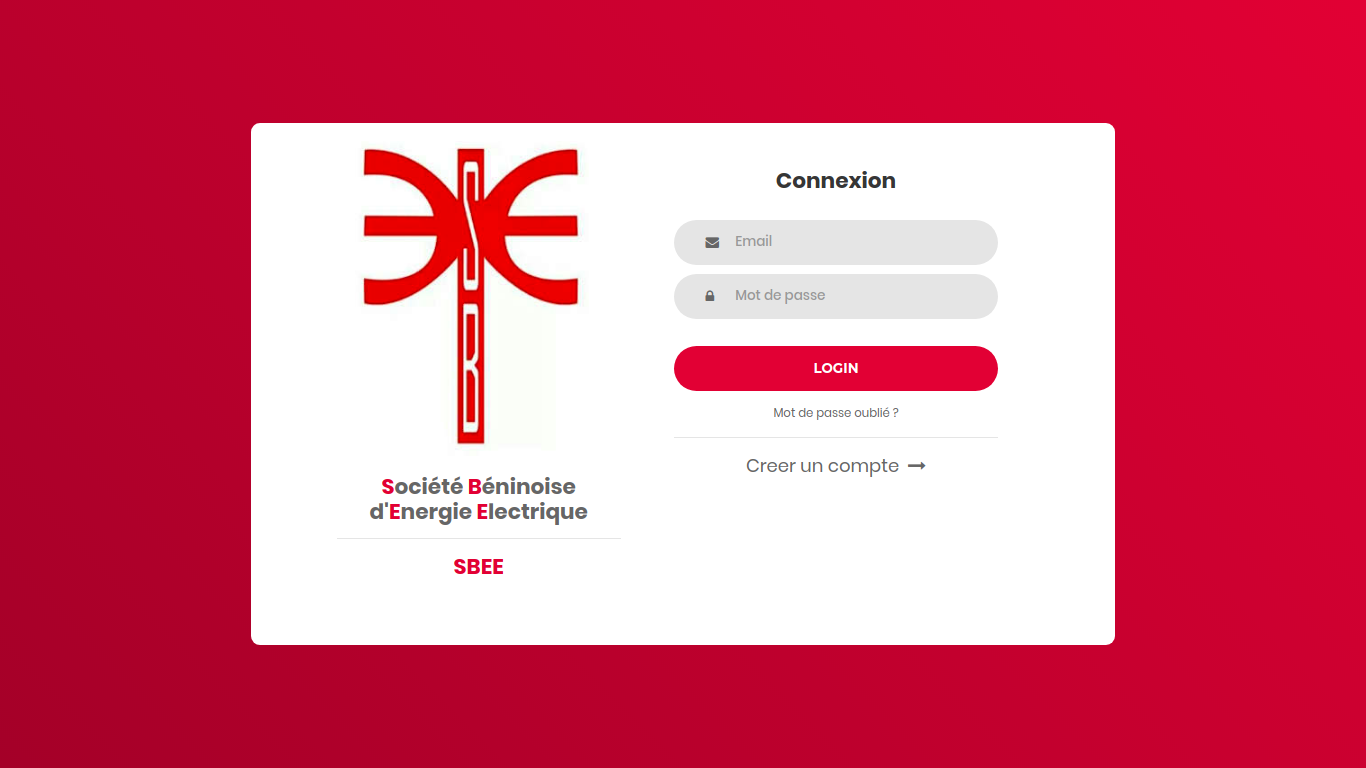
\includegraphics[scale=0.35]{images/login.png}
	      \end{center}
	      \caption{Page de connexion}
	      \label{Page de la whitelist IP}
	  \end{figure}
	  L'utilisateur entre son email et son mot de passe pour se connecter \`a l'application.
      
      \subsection{Interfaces Abonn\'e}
	  \begin{figure}[H]
	      \begin{center}
		  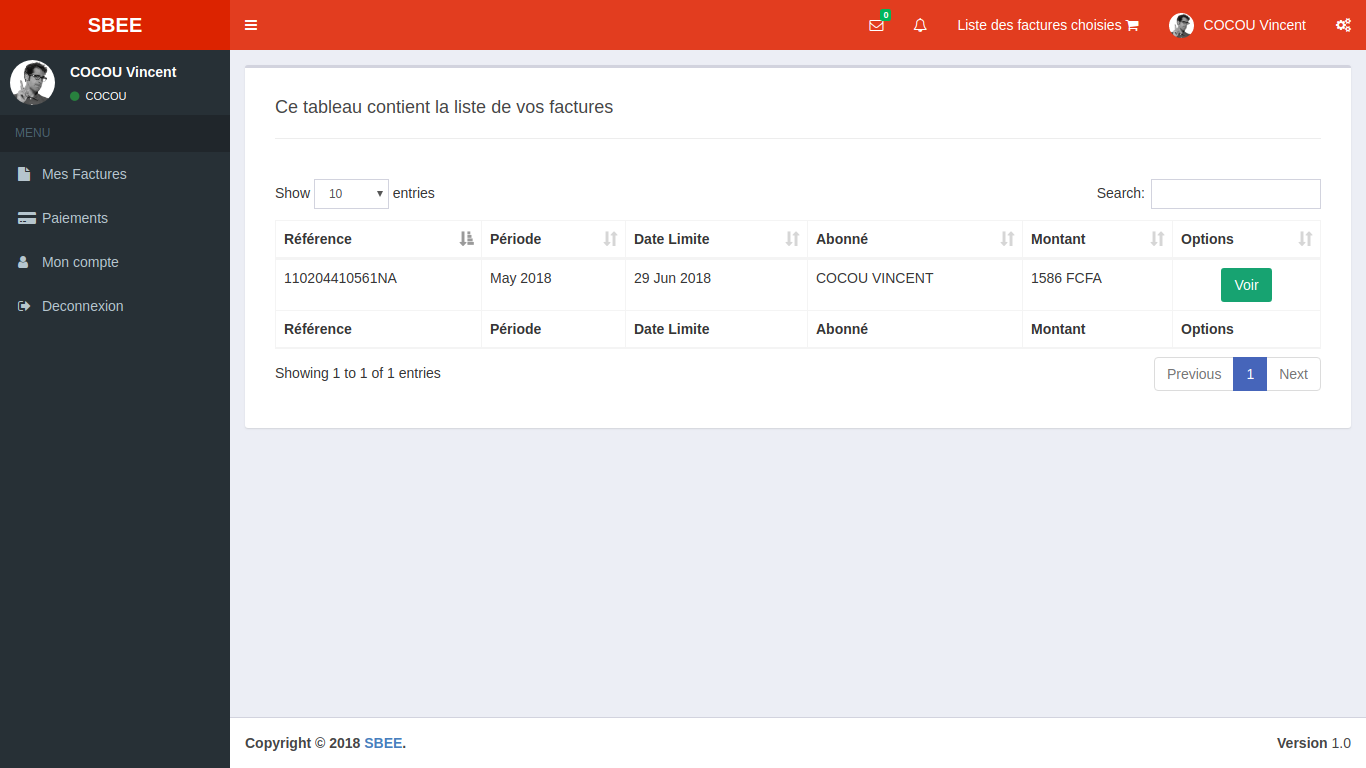
\includegraphics[scale=0.35]{images/listfactures.png}
	      \end{center}
	      \caption{Liste des factures de l'abonn\'e}
	      \label{Page de la whitelist Port}
	  \end{figure}
	  Tous les utilisateurs ont acc\`es \`a la liste de leurs factures. Ils peuvent cliquer sur le bouton \textbf{Voir} pour voir la facture sous le format habituel qu'ils connaissent (le format d'impression et de distribution), ou juste afficher les informations sous forme de liste.
			      
	  \begin{figure}[H]
	      \begin{center}
		  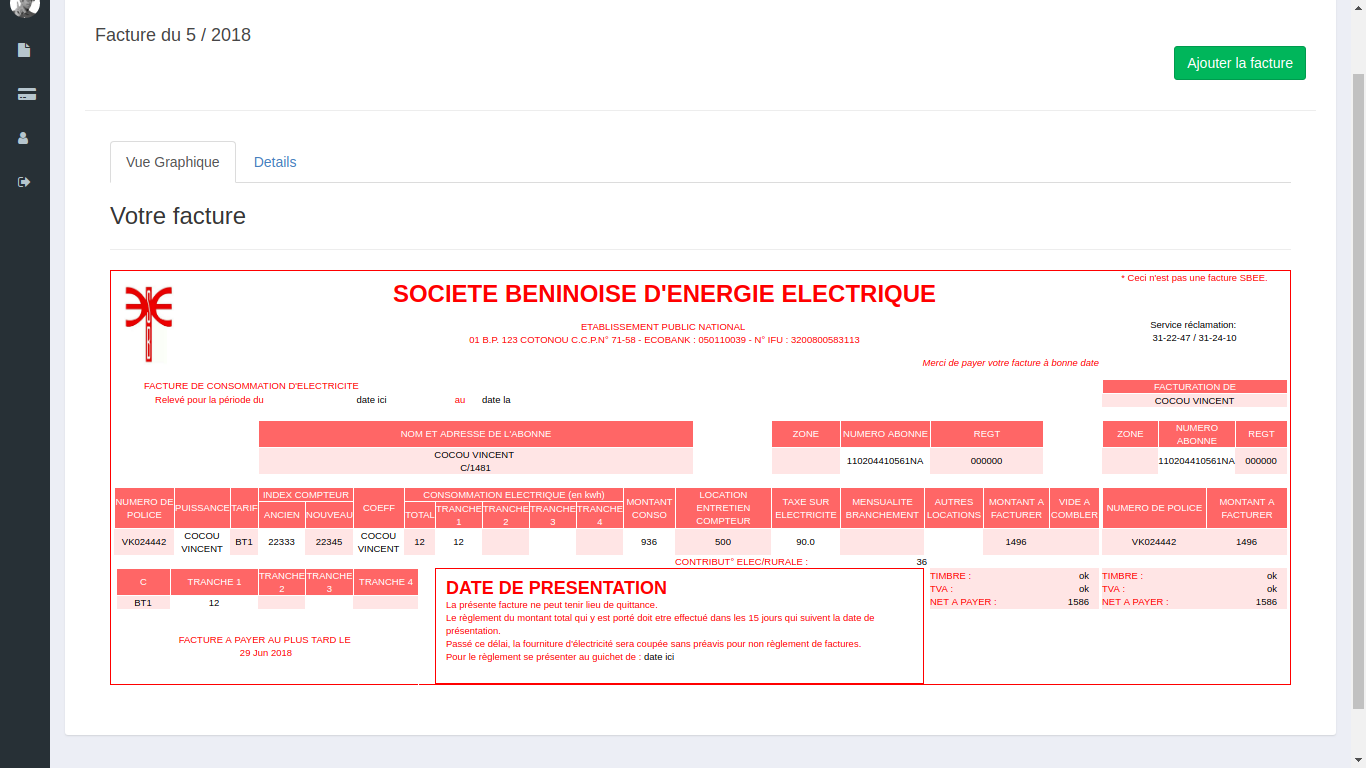
\includegraphics[scale=0.35]{images/graphic.png}
	      \end{center}
	      \caption{Vue d'une facture (Format d'impression)}
	      \label{Page de la whitelist Port}
	  \end{figure}
	  Il s'agit d'une repr\'esentation de la facture physique que nous connaissons tous.
						      
	  \begin{figure}[H]
	      \begin{center}
		  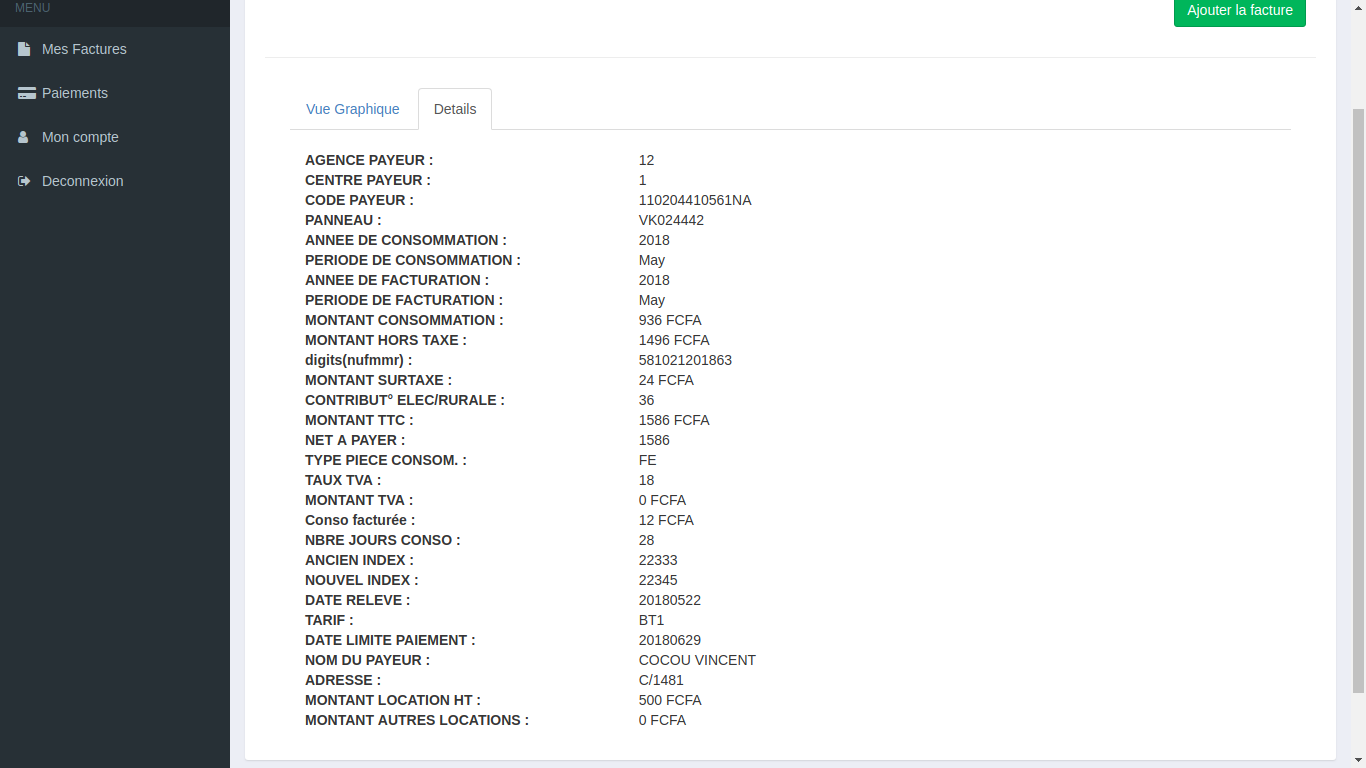
\includegraphics[scale=0.35]{images/details.png}
	      \end{center}
	      \caption{Vue d'une facture (Liste d'informations)}
	      \label{Page de la whitelist Port}
	  \end{figure}
	  Ce format permet d'avoir les informations d'une fa\c{c}on plus lisible et plus claire.
			      
	  \begin{figure}[H]
	      \begin{center}
		  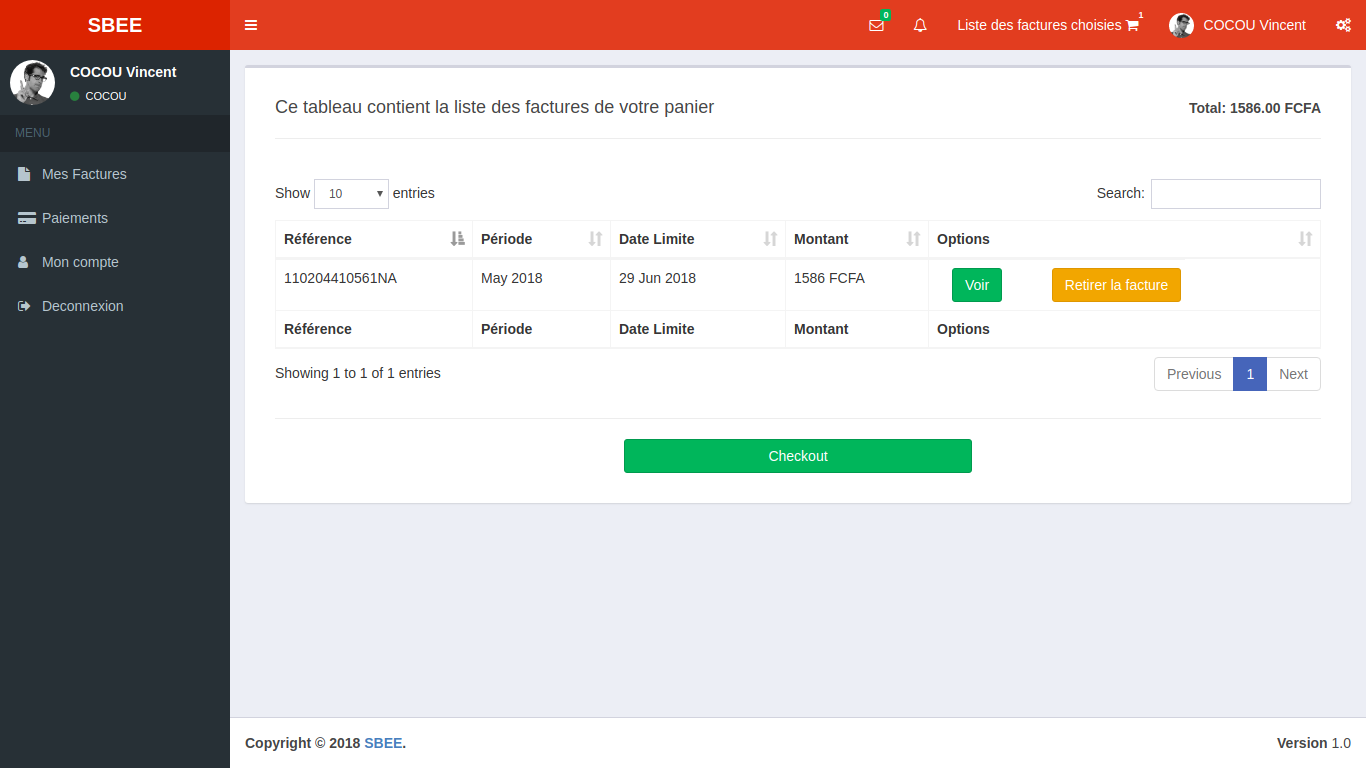
\includegraphics[scale=0.35]{images/choix.png}
	      \end{center}
	      \caption{Liste des factures choisies}
	      \label{Page de la whitelist Port}
	  \end{figure}
	  Afin de permettre de solder plusieurs factures en une fois, l'utilisateur choisit toutes les factures qu'il d\'esire r\'egler et ensuite il proc\`ede au checkout\footnote{Expression anglaise: régler la note, proc\'eder au paiement}.
			      
	  \begin{figure}[H]
	      \begin{center}
		  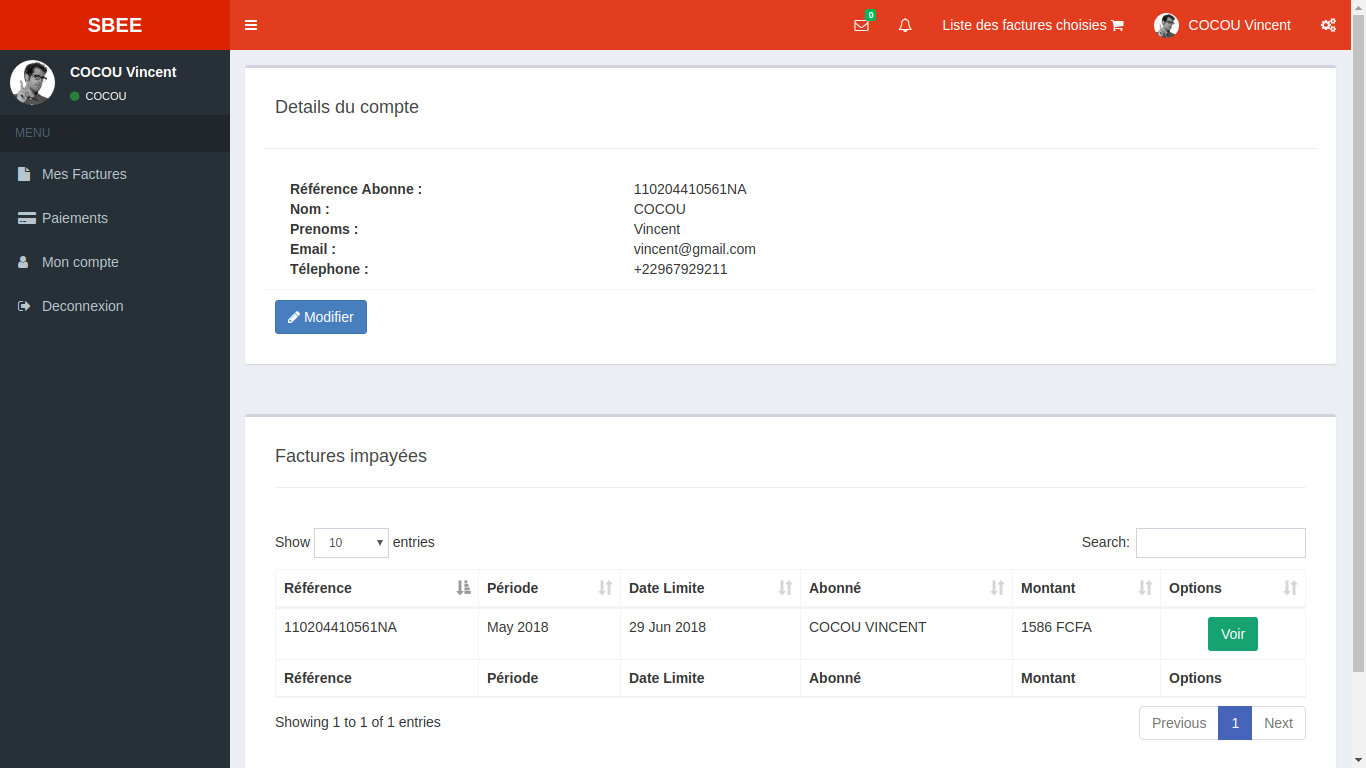
\includegraphics[scale=0.35]{images/detailcompte.png}
	      \end{center}
	      \caption{Le compte d'un utilisateur}
	      \label{Page de la whitelist Port}
	  \end{figure}
	  L'utilisateur a acc\`es aux informations de son compte. Et il peut actuellement modifier son nom, pr\'enom et num\'ero de t\'elephone.
		
      \subsection{Interfaces Administrateurs}
	 Les Administrateurs ont acc\`es \`a bien plus de fonctionnalit\'es que les abonn\'es simples:
	  \begin{itemize}
	    \item La liste des utilisateurs de la plateforme (abonn\'es simples et administrateurs)
	       \begin{figure}[H]
		  \begin{center}
		      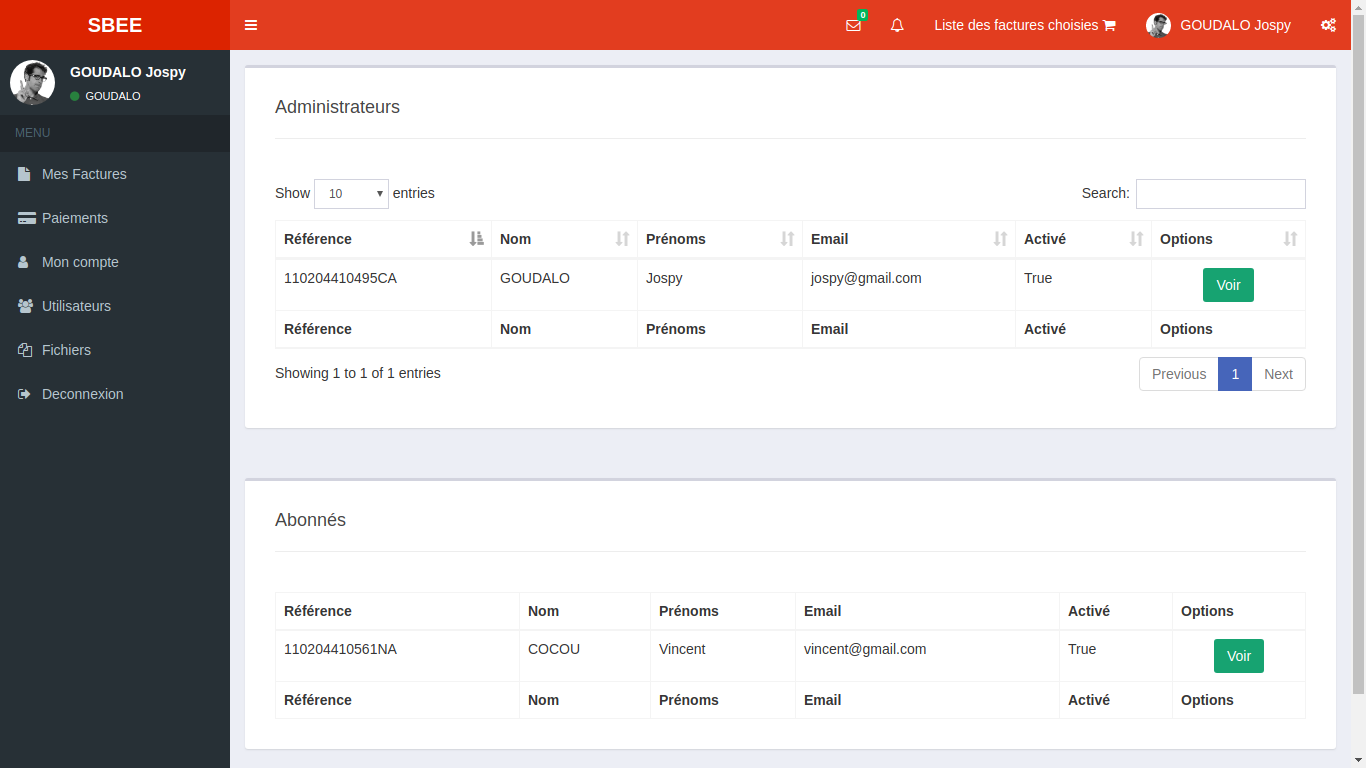
\includegraphics[scale=0.35]{images/gcv.png}
		  \end{center}
		  \caption{Utilisateurs de la plateforme}
		  \label{Page de la whitelist Port}
	      \end{figure}
	    
	    \item Les fichiers: la liste de tous les fichiers factures charg\'es dans la base de données ainsi que les r\`eglements,
	      \begin{figure}[H]
		  \begin{center}
		      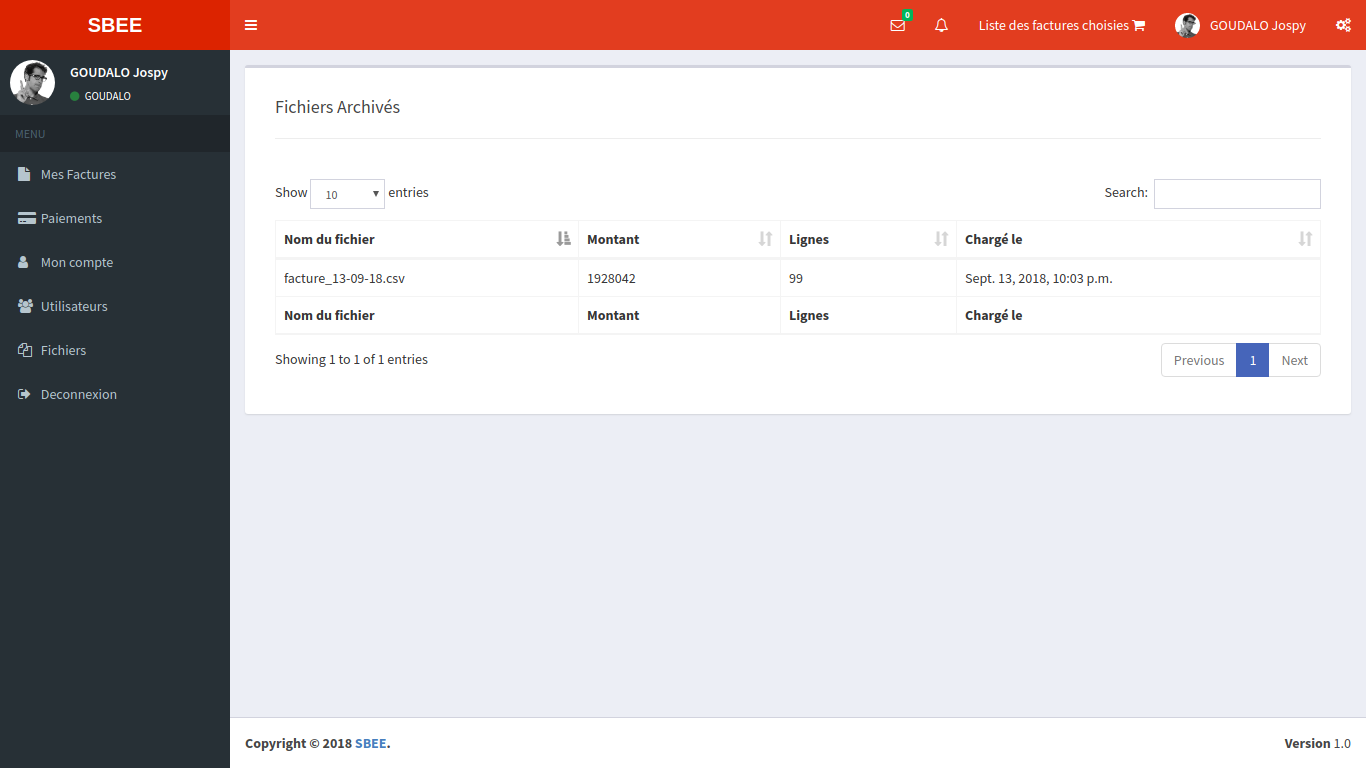
\includegraphics[scale=0.35]{images/files.png}
		  \end{center}
		  \caption{Fichiers import\'es}
		  \label{Page de la whitelist Port}
	      \end{figure}
	      
	  \end{itemize}

	      
    \section{Discussion}
	  \paragraph{}
	      Notre projet est né de plusieurs constats dont entre autre les pertes de temps dans les guichets de la SBEE, et les multiplications croissantes des attaques et intrusions informatiques. Des travaux n'ont pas encore \'et\'e faits \`a l'interne dans les locaux de la SBEE pour palier \`a ces probl\`emes observ\'es. Ceci repr\'esente donc un premier pas fait vers le paiement des factures num\'eriques.
	      
	  \paragraph{}
	      Ainsi, d'une part, notre solution est simple à utiliser et est utilisable depuis un navigateur web. Elle est accessible via internet et ne requiert aucun équipement ou installation spécifique chez l'utilisateur. Elle permet aux utilisateurs de consulter leurs factures et ainsi donc de suivre leur consommation plus facilement. Cependant la soci\'et\'e choisira elle-m\^eme via un appel d'offre ses prestataires pour les diff\'erentes solutions de paiement. Nous avons eu \`a faire quelques recommandations dont: \textbf{Mobile Money de MTN} ainsi que le service mondialement reconnu \textbf{PayPal}.
	      
	  \paragraph{}
	      Aussi existe-t-il des risques de double paiements lors des factures. Etant donn\'e que Gd'Or fonctionne en mode non connect\'e et que les factures ne sont valid\'ees qu`apr\`es 00h, un utilisateur qui va en agence pourrait payer une facture qui a d\'ej\`a \'et\'e pay\'ee en ligne. Cependant ces cas seront rembours\'es par les acteurs des diff\'erentes solutions de paiement car Gd'Or d\'etecte automatiquement les doublures lors de l'apurement des comptes et renvoie des fichiers contenant les erreurs aux entit\'es correspondantes. Celle derni\`ere proc\'edera \`a un remboursement des fonds aux utilisateurs concern\'es.

	  \paragraph{}
	      D'autre part, l'architecture et les outils propos\'es nous permettent d'assurer un minimum de s\'ecurit\'e pour notre application et dans notre r\'eseau. Notre strat\'egie se base essentiellement sur la maitrise du flux de donn\'ees et de la connaissance effective de chaque entit\'e du r\'eseau. Et ceci est un prérequis pour assurer la sécurité : \textbf{On ne protège bien que ce que l’on connaît}. Cependant cette architecture ne nous met pas à l’abri de toutes les attaques, mais nous prot\`ege quand m\^eme contre beaucoup d'attaques courantes, ce qui n’est pas négligeable.

	      
    \section*{Conclusion}
	  \paragraph{}
		  Dans ce chapitre, nous avons exposé les résultats des tests de notre application et réalisé quelques critiques concernant ses performances et ses insuffisances. Ces insuffisances peuvent être perçues comme des perspectives afin d'améliorer le travail fait pour une utilisation plus efficiente.
 	
% \include{perspectives}
%%conclusion
\conclusion
\conclusion
		\paragraph{}
			La sécurité informatique passant par la sécurité de l'information, la sécurité de la vie privée n'est plus aujourd'hui un sujet inconnu. Aussi le hacking constitue-t-il aujourd'hui une arme de guerre assez dévastatrice et silencieuse. Dans cette vision, beaucoup d'outils de sécurité se développent de jour en jour afin de restreindre le champ d'attaque des pirates informatiques qui s'arment davantage. 
		\paragraph{}
			L'objet de ce mémoire a été de mettre en place un système de détection des attaques par webcam et de prévenir par des moyens simples mais efficaces les tentatives d'intrusion. Les solutions proposées proviennent des analyses éffectuées sur les systèmes piratés volontairement. Ainsi les utilisateurs de notre application peuvent être protégés des différentes menaces que nous couvrons.
		\paragraph{}
			Dans ce mémoire, nous avons tout d'abord fait une revue de littérature autour des intrusions informatiques. Nous avons ensuite réalisé la conception de la solution que nous avons proposée avant d'exposer les résultats
			et critiques de l'application que nous avons implémentée.
		\paragraph{}
			Bien que notre solution réponde au besoin énoncé, il faut noter certaines insuffisances telles que 
			l'inactivité de l'application dans les intervalles d'attente.  Bien que cela soit fait pour éviter l'utilisation abusive des ressources du système, il serait préférable de mettre le système en mode écoute. D'une part, un autre axe
			de recherche en ce qui concerne les travaux futurs sera d'explorer la possibilité de rendre 
			l'application accessible sur d'autres plateformes telles que Windows, MAC OS et toutes autres distributions Linux. D'autre part, on pourrait envisager de mettre la recherche de symptômes d'attaques en mode écoute en prenant des mesures autonomes. \cite{ehrig2006graph}
% 
\lhead[]{} \rhead[]{} \chead[]{}

%%biblio
\addcontentsline{toc}{chapter}{Bibliographie}
\bibliographystyle{abbrv}
\bibliography{biblio/biblio}


%\chapter*{Annexe}\addcontentsline{toc}{chapter}{Annexe}\label{annexe1}

\subsection*{Étapes clés du déroulement de l'attaque}


Nous allons exploiter quelques failles de ce réseau pour effectuer une attaque man in the middle (MITM).\\

Au début, notre machine Windows peut atteindre normalement le routeur R4.
\begin{figure}[H]
    \centering
    \includegraphics[scale=0.8]{images/ping_b4_1}
    \caption{Ping vers le routeur R4 avec succès}
    \label{fig:ping_b4_1}
\end{figure}
Quand on essaie de tracer le chemin vers R4, on constate que la machine passe par le routeur R1 légitime du lien pour atteindre R4
\begin{figure}[H]
    \centering
    \includegraphics{images/tracert_b4_1}
    \caption{Traces du chemin vers R4}
    \label{fig:tracert_b41}
\end{figure}
L'attaquant sur le lien peut alors passer a l'attaque.
Pour effectuer l'attaque MITM on utilisera l'outil fake\_router6, un utilitaire du package d'outils \textbf{the hacker choice}.
Ainsi sur la machine d'attaque, on active en un premier lieu le forwarding pour être transparent et ne pas bloquer le transit des paquets.
\begin{figure}[H]
    \centering
    \includegraphics{images/attk/fwrd_activation}
    \caption{Activation du forwarding des paquets.}
    \label{fig:activ_fwrd}
\end{figure}
Aussi on lance wireshark pour observer le trafic des paquets sur notre interface dans le réseau.\\
-------\\
Puisque tout est prêt nous allons lancer l'attaque.

\begin{figure}[H]
    \centering
    \includegraphics[scale=0.8]{images/attk/lancement_attk_1}
    \caption{Initialisation de l'attaque}
    \label{fig:attk_init_1}
\end{figure}

L'attaque est en cours et l'attaquant s'annonce comme le routeur par défaut du lien
nous allons maintenant vérifier la table des routes de notre machine windows.
\begin{figure}[H]
    \centering
    \includegraphics{images/attk/tableRoutes_windows}
    \caption{Table des routes de la machine victime}
    \label{fig:win_route_table}
\end{figure}
On constate que l'attaquant s'est insère comme passerelle de la victime.
pour confirmer cela reprenons un tracert vers le routeur r4
\begin{figure}[H]
    \centering
    \includegraphics{images/attk/tracert_b4_2}
    \caption{Chemin vers b4 pendant l'attaque.}
    \label{fig:tracert_b42}
\end{figure}
On peut voir clairement que la victime passe par l'attaquant pour atteindre le routeur.\\

A présent nous allons essayer de capturer une information envoyée par la victime.
Pour cela la victime fait un telnet sur le router R4 pour s'y connecter avec les paramètres suivants:\\
password1:\textbf{cisco}\\
password2:\textbf{class}
\begin{figure}[H]
    \centering
    \includegraphics{images/attk/telnet_r4}
    \caption{Connexion telnet au routeur.}
    \label{fig:telnetr4}
\end{figure}

Une fois la connexion réussie, nous allons voir avec wireshark les paquets de connexion et y retrouver les paramètres de connexion.
\begin{figure}[H]
    \centering
    \includegraphics[width=1.0\textwidth]{images/attk/c}
    \includegraphics[width=1.0\textwidth]{images/attk/i}
    \includegraphics[width=1.0\textwidth]{images/attk/s}
    \includegraphics[width=1.0\textwidth]{images/attk/c2}
    \includegraphics[width=1.0\textwidth]{images/attk/o}   
    \caption{Premier paramètre de connexion au routeur R4: \textbf{c-i-s-c-o}}
    \label{fig:param_conn_r4}
\end{figure}
\begin{figure}[H]
    \centering
    \includegraphics[width=1.0\textwidth]{images/attk/param2_c}
    \includegraphics[width=1.0\textwidth]{images/attk/param2_l}
    \includegraphics[width=1.0\textwidth]{images/attk/param2_a}
    \includegraphics[width=1.0\textwidth]{images/attk/param2_s1}
    \includegraphics[width=1.0\textwidth]{images/attk/param2_s2}
    \caption{Second paramètre de connexion au routeur R4: \textbf{c-l-a-s-s}}
    \label{fig:param_conn2}
\end{figure}
Les paramètres on été retrouves donc l'attaque a été un succès!

%\subsection*{Mitigations}
%Pour sécuriser ce réseau afin d'éviter ce genre d'attaque, deux mesures de sécurité peuvent être configurées.
%\begin{itemize}
%    \item le SEND
%    \item le RaGuard
%\end{itemize}


\end{document}          
